% -- Titulo e Descricao ------------------------------------------------------
\newcommand{\tittese}{%
	\textsf{\bfseries\Large Verifica��o de programas C++ baseados no \textit{framework} cross-plataforma Qt\\
	\vspace{0.8ex}
        }}

\newcommand{\descrtese}{%
\hspace{\stretch{1}}\parbox{0.51\textwidth}{%
Disserta��o apresentada ao Programa de P\'os-Gradua\c{c}\~ao em Engenharia El�trica, como requisito parcial
para obten\c{c}\~ao do T\'{\i}tulo de Mestre em Engenharia El�trica. \'Area de concentra\c{c}\~ao: Controle e Automa��o de Sistemas.
}}

% -- Capa ---------------------------------------------------------------------

\frontmatter
%\doublespacing
%\singlespacing
\pagestyle{empty}

%{centering
\begin{center}

\includegraphics[bb=0 0 646 638,height=2.5cm]{figuras/ufam.png}

\textsf{\large%
Universidade Federal do Amazonas\\
Faculdade de Tecnologia\\
Programa de P\'os-Gradua\c{c}\~ao em Engenharia El�trica}

\vspace*{4cm}
\vspace*{\stretch{1}}

\tittese

\vspace*{4cm}
\vspace*{\stretch{1}}

{\large M�rio Angel Praia Garcia}

\vspace*{3cm}
\vspace*{\stretch{1}}

Manaus -- Amazonas

Agosto de 2016
\end{center}

%}
%\cleardoublepage


% -- Contracapa ---------------------------------------------------------------

%{\singlespacing\centering
\begin{center}
{\large M�rio Angel Praia Garcia}

\vspace*{4cm}
\vspace*{\stretch{2}}

\tittese

\vspace*{2cm}
\vspace*{\stretch{1}}

\descrtese

\vspace*{2cm}
\vspace*{\stretch{1}}

Orientador: Lucas Carvalho Cordeiro \\
Coorientador: Waldir Sabino da Silva J�nior
\end{center}

%}
%\cleardoublepage

% -- Ficha Catalografica ------------------------------------------------------

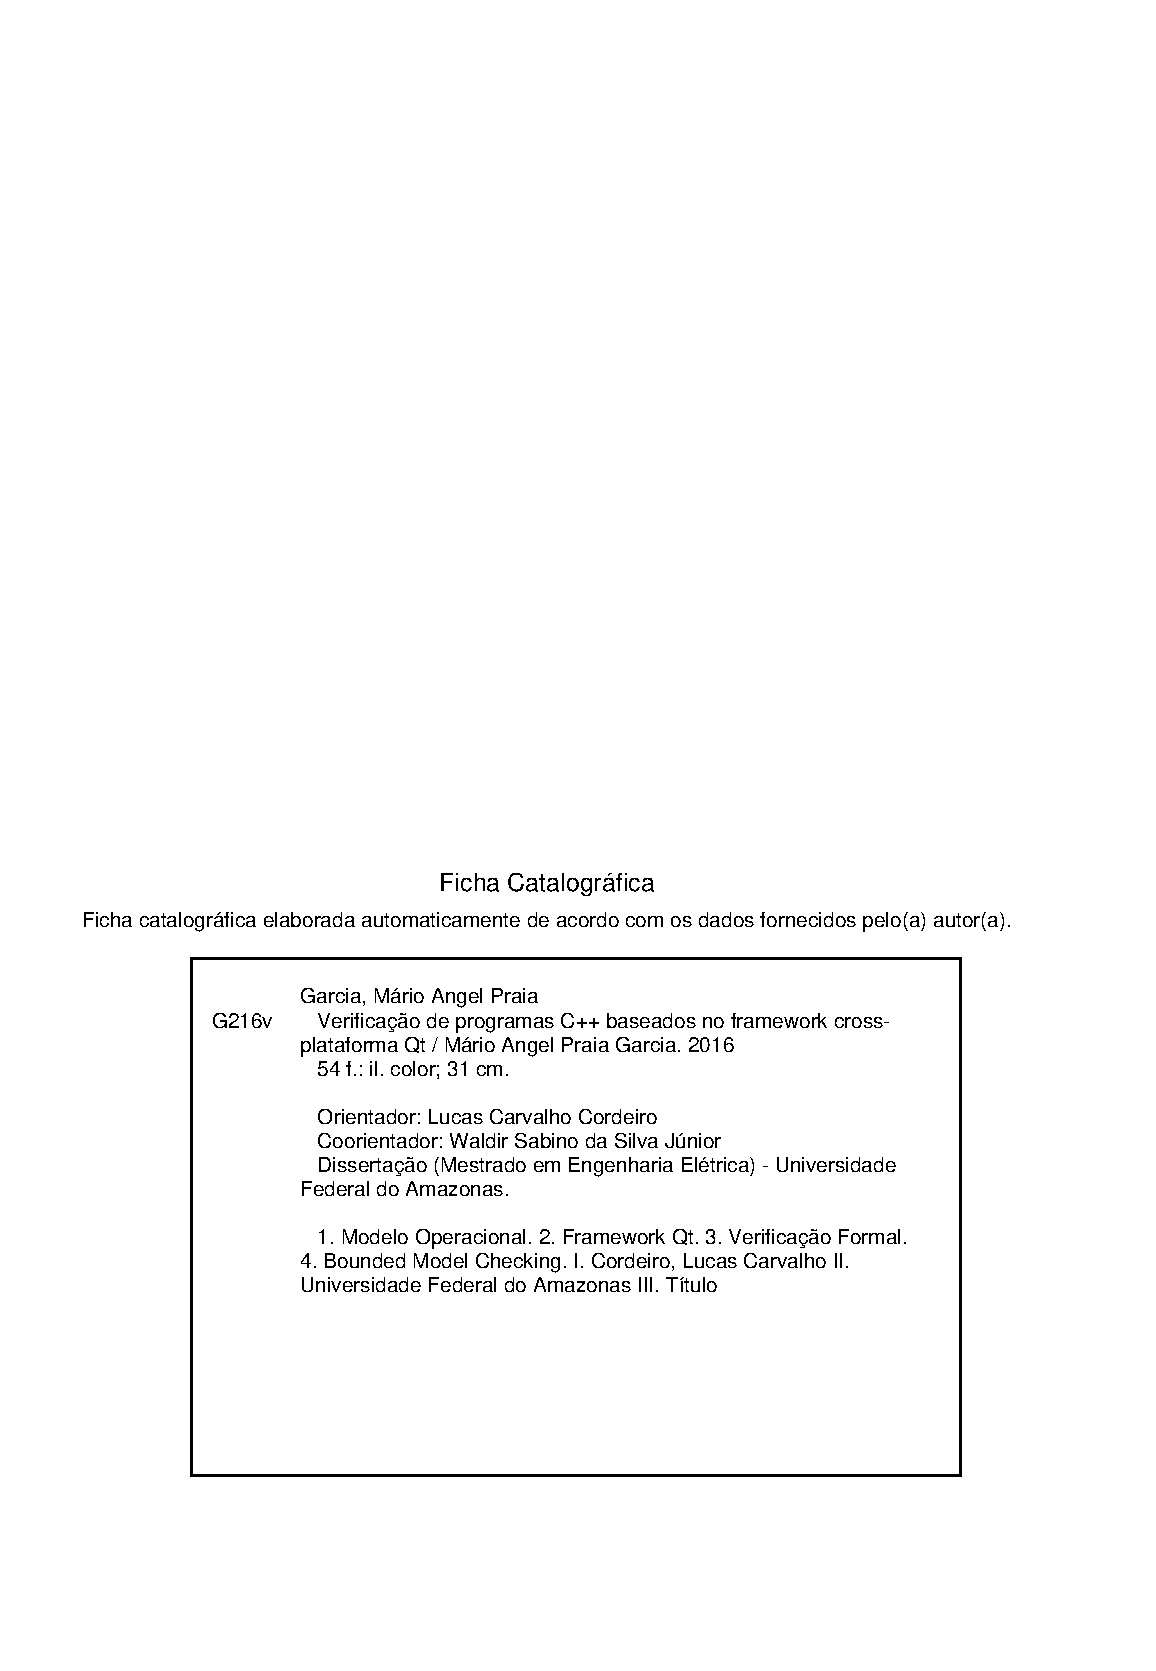
\includepdf[pages=-]{fichacat/fichaCatalografica.pdf}

% -- Banca Examinadora --------------------------------------------------------

%{\singlespacing\centering

\begin{center}
{\large M�rio Angel Praia Garcia}

\vspace*{2cm}
%\vspace*{\stretch{2}}
{\large Verifica��o de programas C++ baseados no \textit{framework} cross-plataforma Qt}
%\tittese

\vspace*{2cm}
%\vspace*{\stretch{1}}

\descrtese

\vspace*{1cm}
%\vspace*{\stretch{1}}

\begin{flushleft}
Aprovado em 13 de setembro de 2016
\end{flushleft}
\vspace*{1cm}

{\large Banca Examinadora}
\vspace{3em}

Prof. D.Sc. Waldir Sabino da Silva J�nior -- Presidente e Coorientador\\
Departamento de Eletr�nica e Computa��o -- UFAM
\vspace{3em}

Prof. D.Sc. Raimundo da Silva Barreto -- Membro \\
Instituto de Computa��o -- UFAM
\vspace{3em}

Prof. D.Sc. Tayana Uch�a Conte -- Membro \\
Instituto de Computa��o -- UFAM
\vspace{2em}

%\vspace*{1cm}
\vspace*{\stretch{0.5}}

Manaus -- Amazonas

\end{center}
%}
\cleardoublepage
